\documentclass[12pt, psamsfonts]{amsart}

%-------Packages---------
\usepackage{amssymb,amsfonts}
\usepackage{fullpage}
\usepackage{todonotes}
\usepackage{physics}
\usepackage[all,arc]{xy}
\usepackage{enumerate}
\usepackage{mathrsfs}
\usepackage{theoremref}
\usepackage{graphicx}
\usepackage[bookmarks]{hyperref}

%--------Theorem Environments--------
%theoremstyle{plain} --- default
\newtheorem{thm}{Theorem}[section]
\newtheorem{cor}[thm]{Corollary}
\newtheorem{prop}[thm]{Proposition}
\newtheorem{lem}[thm]{Lemma}
\newtheorem{conj}[thm]{Conjecture}
\newtheorem{quest}[thm]{Question}

\theoremstyle{definition}
\newtheorem{defn}[thm]{Definition}
\newtheorem{defns}[thm]{Definitions}
\newtheorem{con}[thm]{Construction}
\newtheorem{exmp}[thm]{Example}
\newtheorem{exmps}[thm]{Examples}
\newtheorem{notn}[thm]{Notation}
\newtheorem{notns}[thm]{Notations}
\newtheorem{addm}[thm]{Addendum}
\newtheorem*{exer}{Exercise}

\theoremstyle{remark}
\newtheorem{rem}[thm]{Remark}
\newtheorem{rems}[thm]{Remarks}
\newtheorem{warn}[thm]{Warning}
\newtheorem{sch}[thm]{Scholium}

\DeclareMathOperator{\Hom}{Hom}
\DeclareMathOperator{\Id}{Id}

\makeatletter
\let\c@equation\c@thm
\makeatother
\numberwithin{equation}{section}

\bibliographystyle{plain}

\begin{document}

\title{Math 611 Homework (Due 9/18)}
\author{Hidenori Shinohara}
\maketitle


\begin{exer}{(Problem 12, Chapter 1.2)}
  The Klein bottle is usually pictured as a subspace of $\mathbb{R}^3$ like the subspace $X \subset \mathbb{R}^3$ shown in the first figure at the right.
  If one wanted a model that could actually function as a bottle, one would delete the open disk bounded by the circle of self-intersection of $X$, producing a subspace $Y \subset X$.
  Show that $\pi_1(X) \approx \mathbb{Z} * \mathbb{Z}$ and that $\pi_1(Y)$ has the presentation $\langle a, b, c \mid aba^{-1}b^{-1}cb^{\epsilon}c^{-1} \rangle$ for $\epsilon = \pm 1$.
  Show also that $\pi_1(Y)$ is isomorphic to $\pi_1(\mathbb{R}^3 \setminus Z)$ for $Z$ the graph shown in the figure.
\end{exer}

\begin{proof}
  We will construct $X$ from the 1-skeleton in Figure \ref{fig:fund_x_klein}.
  \begin{figure}
    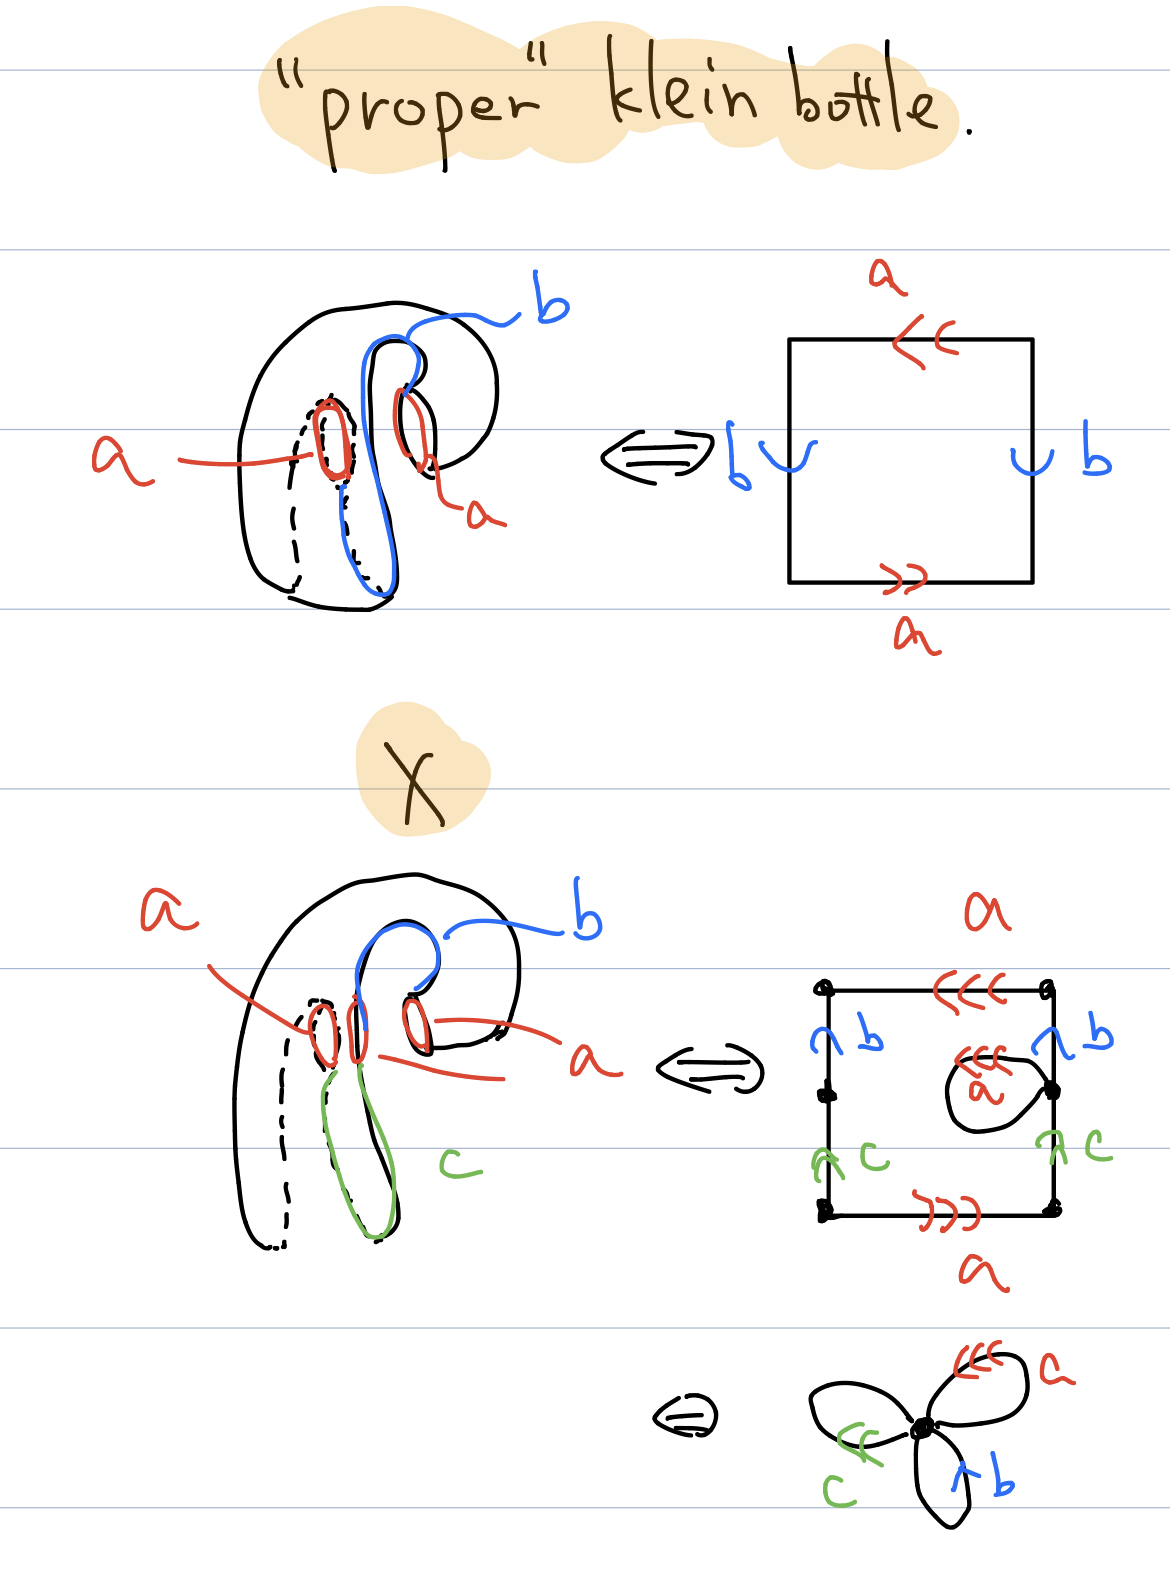
\includegraphics[width=.5\linewidth]{klein_solution_zz.jpeg}
      \caption{Fundamental Group of $X$}
    \label{fig:fund_x_klein}
  \end{figure}
  The 1-skeleton has three loops $a, b, c$, so the fundamental group is $\langle a, b, c \mid \rangle$.
  The main difference between $X$ and the ``proper" Klein bottle is that the loop $a$ actually gets glued on the surface.
  Thus we will glue the first 2-cell to around $a$, and another 2-cell on the loop $c^{-1}acbab^{-1}$.
  Therefore, we end up with the fundamental group $\langle a, b, c \mid a, c^{-1}acabab^{-1} \rangle$.
  Then $\langle a, b, c \mid a, c^{-1}acabab^{-1} \rangle \approx \langle b, c \mid \rangle \approx \mathbb{Z} * \mathbb{Z}$ since the relation $c^{-1}acabab^{-1}$ is trivial.
  \todo[inline]{
    Getting rid of $a$ from the relation gives something similar to the problem.
    $ba^{-1}b^{-1}a^?c^{-1}a^{-1}c$.
    I'm not sure what the orientation of $a$ should be.
    (I think this actually affects the first part too...
  }

\end{proof}

\begin{exer}{(Problem 14, Chapter 1.2)}
  Consider the quotient space of a cube $I^3$ obtained by identifying each square face with the opposite square face via the right-handed screw motion consisting of a translation by one unit in the direction perpendicular to the face combined with a one-quarter twist of the face about its center point.
  Show this quotient space $X$ is a cell complex with two 0-cells, four 1-cells, three 2-cells, and one 3-cell.
  Using this structure, show that $\pi_1(X)$ is the quaternion group $\{ \pm 1, \pm i, \pm j, \pm k \}$ of order eight.
\end{exer}

\begin{proof}
  \begin{figure}
    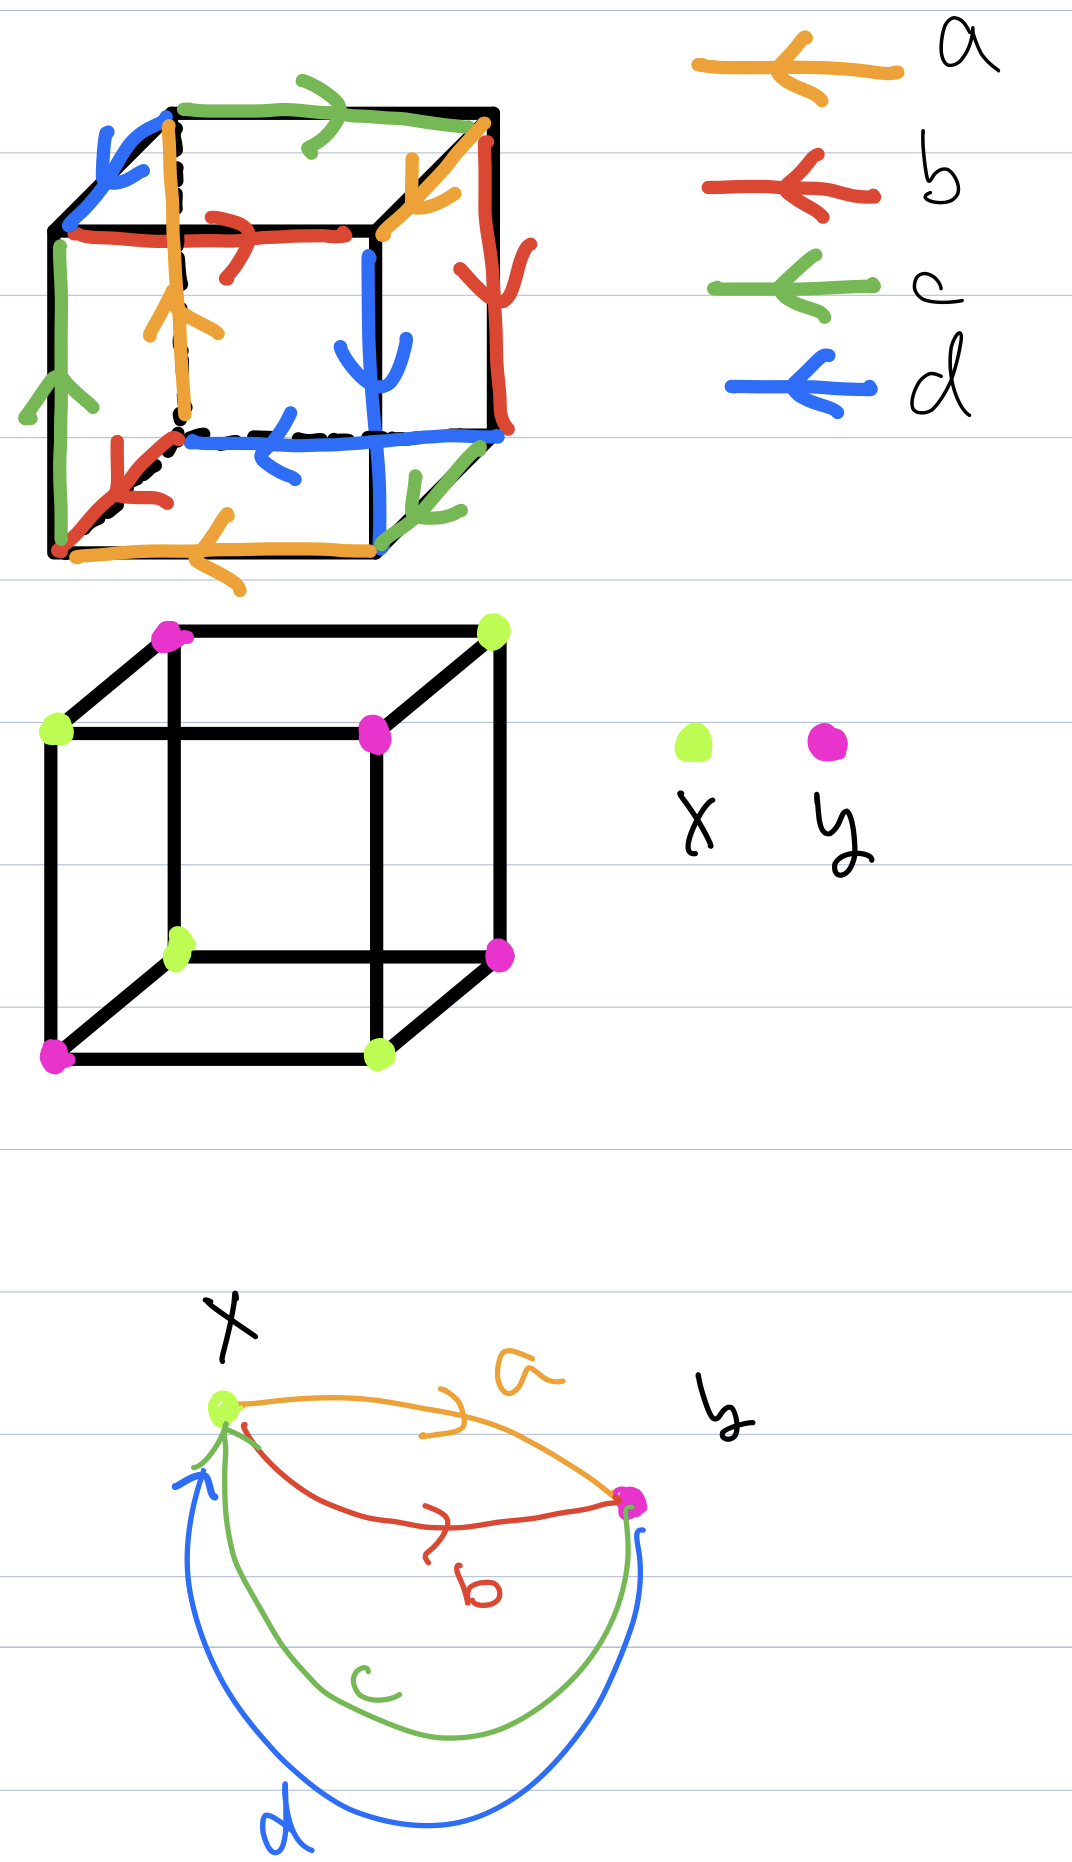
\includegraphics[width=.5\linewidth]{cube.jpeg}
    \caption{Problem 14}
    \label{fig:cube}
  \end{figure}
  The vertices and edges get identified as in Figure \ref{fig:cube}.
  Thus we have two 0-cells and four 1-cells.
  Since the opposite faces are identified and the cube has 6 faces, we need to glue three 2-cells to the cube.
  Lastly, we need a 3-cell glued to the three faces.
  By Proposition 1.26, the fundamental group of a 2-skeleton is the same as the fundamental group of a space obtained by attaching 3-cells, so it suffices to consider the fundamental group we obtain by attaching the three 2-cells to the graph.
  As in Figure \ref{fig:cube}, the graph has 4 edges between two vertices.
  The fundamental group of this is $\langle ab^{-1}, ac, ad \rangle$ because by ``shrinking" $a$ we obtain the graph consisting of one vertex and three loops.
  By attaching a 2-cell to each of the top-bottom pair, left-right pair, and the front-back pair, we obtain

  \begin{align*}
    \langle ab^{-1}, ac, ad \mid ab^{-1}d^{-1}c, adc^{-1}b^{-1}, acbd \rangle.
  \end{align*}

  Thus this is the fundamental group of the given space.

  \todo[inline]{
    Prove that $i^2 = j^2 = k^2 = ijk$ where $i = ac$ and $j = ab^{-1}$ and $k = ad$.
    I have already finished it in the notes.
    I think I need to show that $i^2 \ne e$ and $i^4 = e$, but I have no idea how.
  }

\end{proof}

\end{document}


